Debido al gran tama\~no del diagrama, lo separamos en dos fragmentos de manera de hacerlo m\'as legible. Ambas partes pueden leerse de manera independiente y est\'an centradas en la entidad Legislador.
			
		\begin{figure}[H]
		  \begin{center}
		    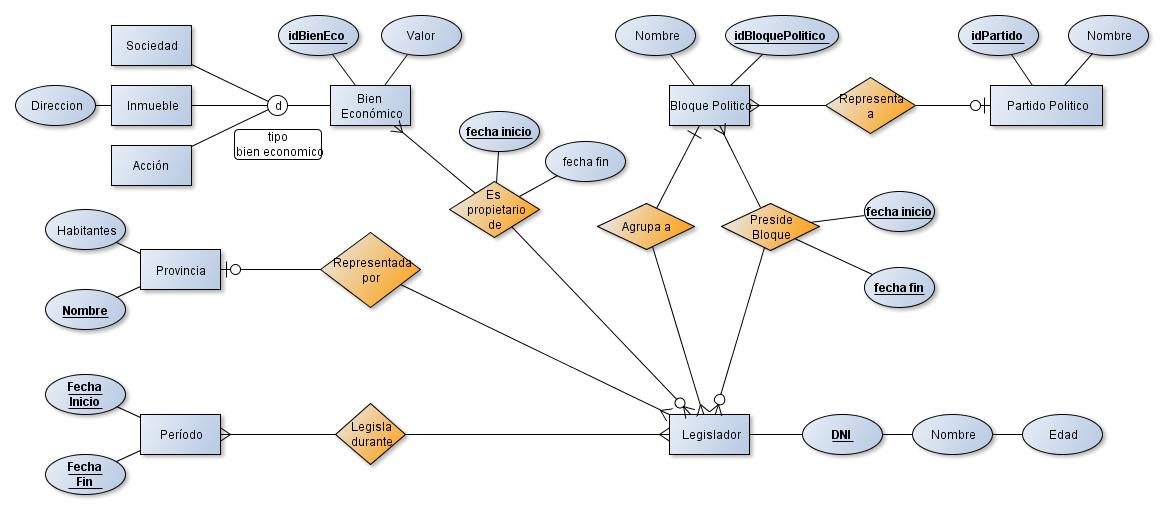
\includegraphics[scale=.40,angle=90]{./imagenes/DER2-arriba.jpg}
		    \caption{fragmento der} 
		    \label{fig:derparte1}
		  \end{center}
		\end{figure}
				
		\begin{figure}[H]
		  \begin{center}
		    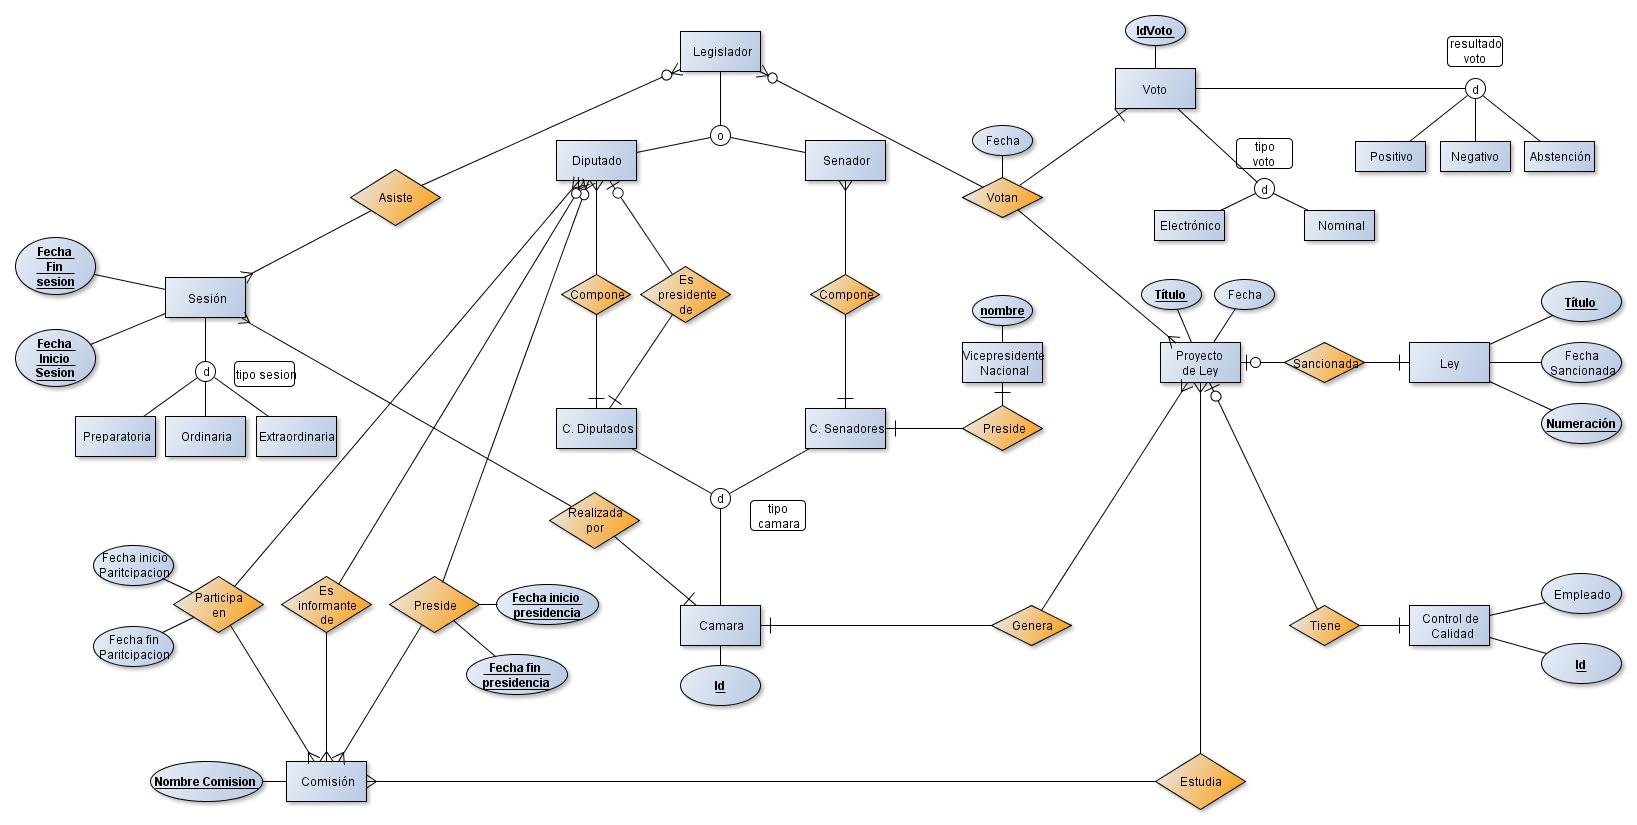
\includegraphics[scale=.35,angle=90]{./imagenes/DER2-abajo.jpg}
		    \caption{fragmento der segunda parte} 
		    \label{fig:derparte2}
		  \end{center}
		\end{figure}